% TLDR: TMLR version built only from the VeriBench launch page's language-model judge section: an audit of one judge's agreement with human ratings of formal specification coverage.
\documentclass[10pt]{article}
% Anonymous double-blind submission; [preprint] de-anonymizes, [accepted] is for the camera-ready version.
\usepackage{tmlr}
\usepackage{hyperref}
\usepackage{url}
\usepackage{booktabs}
\usepackage{amsmath,amssymb}
\usepackage{graphicx}
% Point estimate with its 95% interval underneath, for tables.
\newcommand{\est}[3]{\begin{tabular}[t]{@{}c@{}}#1\\[-2pt]{\scriptsize[#2, #3]}\end{tabular}}

\title{What a Single Correlation Hides: Auditing a Language-Model Judge of Formal Specification Coverage}
\author{Anonymous authors}

\begin{document}
\maketitle
% !TEX root = 00_main.tex
% TLDR: One reported judge--human correlation hides uncertainty, rank and level disagreement, target dependence and mismatched judge inputs.
% Provenance for every number: experiments/archive/19_audit_gpt_5_3_codex_rubric_judge_on_75_rated_outputs_start_12Nov2026_end_12Nov2026/POSTHOC_CLI_RUBRIC_JUDGE_AGREEMENT_11-12-2026.json (post hoc, 11-12-2026), which reproduces the receipt values r=0.6137, rho=0.3755 to 1e-12.
\begin{abstract}
% CS197 move 1: problem motivation (failure mode) -- coverage scores depend on an LLM judge.
Lean~4 formalization benchmarks use language-model judges to score whether an agent's theorem statements cover a human-written reference.
% CS197 move 2: assumption (setup bit) -- one correlation with human ratings is taken to validate the judge.
Such a judge is often justified by one correlation between its scores and human ratings.
% CS197 move 3: contribution (bit flip) -- audit the reported correlation rather than report it.
We audit one such justification, a reported Pearson correlation of 0.61, and show what the single coefficient leaves out.
% CS197 move 4a: instantiation (bit flip instantiation) -- same artifacts, shared rubric.
A GPT-5.3-Codex judge scored 75 Lean artifacts from 25 tasks that five human raters had rated under a shared 0--5 coverage rubric.
% CS197 move 4b: instantiation (bit flip instantiation) -- existing scores only; task resampling, absolute agreement, input check.
We reanalyze the saved scores with task-level resampling, rank and absolute agreement, and a byte-level check of the judge's inputs.
% CS197 move 5a: evaluation (headline numbers) -- uncertainty and rank; item-level, pooled target.
The correlation's 95\% task-bootstrap interval is [0.21, 0.82], and Spearman correlation is 0.38.
% CS197 move 5b: evaluation (diagnostic result) -- level; mean bias -0.825 on 0-5, judge minus pooled human mean.
The judge also rates artifacts 0.83 points below the human mean on the 0--5 scale.
% CS197 move 5c: evaluation (diagnostic result) -- target; experiment 58 label-group receipt, point estimates.
Against lenient raters the correlation is 0.70; against expert raters it is 0.37.
% CS197 move 5d: evaluation (diagnostic result) -- inputs; judge_reference_statements_match_rating_era subset, rho=0.564956.
For 24 artifacts the judge's reference theorems differ from those the raters saw.
On the other 51, Spearman correlation is 0.56.
% CS197 move 5e: evaluation (diagnostic result) -- isotonic remapping, out of fold: bias -0.018, rho=0.046.
A supervised score remapping removes the offset but also nearly all association.
% CS197 move 6: implication (north star) -- from one coefficient to an auditable measurement.
We recommend that coverage-judge audits report task-level intervals, rank and absolute agreement, the rater target, and whether the judge saw the raters' inputs.
\end{abstract}
% Alternate opening A (failure-mode-first): A language-model judge can correlate with human ratings of Lean theorems while ranking them differently, rating them lower and reading different references.
% Alternate opening B (contrast-first): A judge's correlation of 0.61 with human raters can mean anything from strong agreement to almost none, depending on what the coefficient averages over.
% Alternate opening C (question-first): What does a single judge--human correlation establish about a language-model judge of theorem coverage?

% !TEX root = 00_main.tex
% TLDR: A reported judge--human correlation is a measurement to audit; the audit changes what it supports.
\section{Introduction}
\label{sec:intro}
% CS197 move 1: problem motivation -- proofs can succeed while required properties are missing; coverage needs a judge.
A Lean file can compile, and even prove every theorem it states, while omitting properties that its source program must satisfy.
Benchmarks that ask coding agents to formalize programs therefore score \emph{formal specification coverage}.
It measures how fully the agent's theorem statements express the obligations in a human-written reference.
% Provenance: public VeriBench report (TE1, theorem equivalence; SCSC product) and launch page ("Theorem coverage (TC1)").
\textsc{VeriBench} calls this quantity theorem equivalence (TE1) in its report and theorem coverage (TC1) on its launch page~\citep{veribench2026}.
Establishing coverage formally requires proving implications between statements, which is itself a hard proof task.
Such benchmarks delegate the coverage score to a language-model judge instead.
Because that score is one factor of the benchmark's multiplicative overall score~\citep{veribench2026}, the judge's agreement with expert judgment shapes what the benchmark measures.

% CS197 move 2: assumption -- one correlation with human ratings validates a judge.
Language-model judges are usually justified by their agreement with human ratings~\citep{zheng2023judging,liu2023geval,chiang2023can}.
That agreement is often summarized by a single correlation coefficient.
A correlation measures association rather than agreement: a method can correlate with a reference while reading consistently higher or lower~\citep{bland1986statistical}.
Its value also depends on choices that the coefficient does not record.
These include how ratings are grouped, which raters define the target, and whether the judge read the same inputs as the raters.

% CS197 move 3: contribution -- audit the reported number instead of accepting it.
We treat a reported judge--human correlation as a measurement to audit rather than a number to accept.
Our object is the evidence behind one benchmark launch claim.
\textsc{VeriBench} reports that a GPT-5.3-Codex judge given the raters' rubric reaches Pearson correlation $r=0.6137$ against its human ratings, with weaker rank correlations~\citep{veribench2026}.
It presents this result as an alignment check, not as evidence that its deployed coverage scorer was fitted to human ratings.
We ask what the reported number establishes about the judge.

% CS197 move 4: instantiation -- reanalysis of archived receipts with task resampling, absolute agreement, targets and an input check.
We reanalyze the archived per-artifact scores of that judge and the human ratings it was compared with, without new model calls or new ratings.
The data are 75 Lean artifacts from 25 tasks.
Five raters rated them on a 0--5 coverage rubric, and the judge scored each artifact three times.
We complement the reported coefficient with intervals that resample tasks and with rank and absolute agreement.
We also separate within-task from between-task correlation, vary the rater target, and hash-compare the judge's inputs with the rated files (Figure~\ref{fig:intervals}).

% CS197 move 5: evaluation -- headline numbers; POSTHOC_CLI_RUBRIC_JUDGE_AGREEMENT_11-12-2026.json.
The reported correlation reproduces exactly, but its 95\% interval over tasks is [0.213, 0.821], and Spearman correlation is 0.375 [0.013, 0.668].
The judge rates artifacts 0.825 points below the human mean on the 0--5 scale.
Its absolute-agreement intraclass correlation, 0.429, therefore falls well below its consistency intraclass correlation, 0.613.
After centering scores within each task, Pearson correlation drops to 0.358 [0.055, 0.635].
The Spearman correlation computed inside each task averages only 0.255 [$-0.073$, 0.579].
The same judge scores have Pearson correlation 0.702 with the mean of lenient raters and 0.372 with the mean of expert raters.
For eight of the 25 tasks, the judge's reference theorems differ from those the raters saw.
On the other 17 tasks, Spearman correlation is 0.565 [0.197, 0.800], but the downward offset remains.
A supervised isotonic remapping removes the offset but leaves Spearman correlation at 0.046, and its absolute error is close to that of a constant prediction.

% CS197 move 6: implications and contributions -- no verdict on validity from one coefficient; checklist.
These results neither validate nor reject the judge; they show that the reported coefficient alone cannot tell which.
They also concern a different judge from the one that produced the benchmark's reported coverage scores, which used another model and rubric~\citep{veribench2026}.
We make the following contributions:
\begin{enumerate}
\item We reconstruct the evidence behind a reported judge--human correlation for formal specification coverage and reproduce it exactly from archived receipts.
\item We show that task-level uncertainty, rank and absolute agreement, the choice of rater target, and mismatched judge inputs each change what the correlation supports, with task-bootstrap intervals for every statistic we derive against the pooled target.
\item We derive a short reporting checklist for audits of coverage judges from these findings.
\end{enumerate}

\begin{figure}[t]
\centering
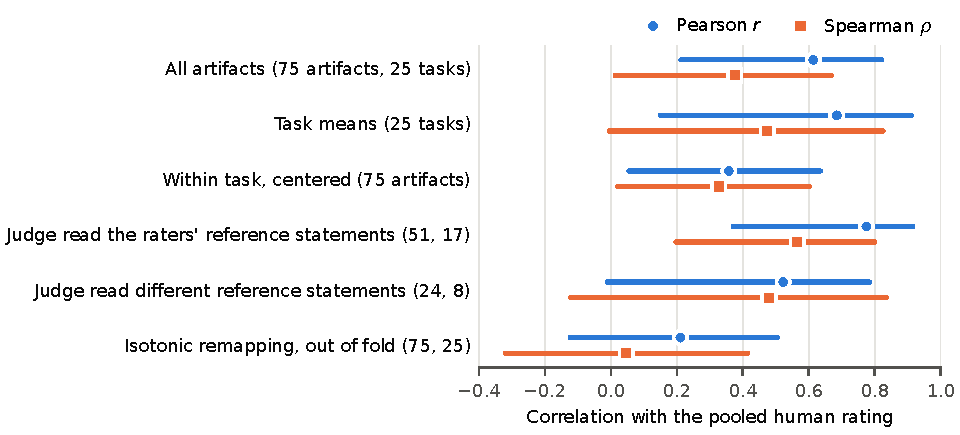
\includegraphics[width=\linewidth]{figures/agreement_intervals.pdf}
% Provenance: figures/make_agreement_figure.py reads POSTHOC_CLI_RUBRIC_JUDGE_AGREEMENT_11-12-2026.json; aggregates only.
\caption{\textbf{The same judge scores give correlations from near zero to 0.77, depending on how agreement is computed.} Pearson $r$ (circles) and Spearman $\rho$ (squares) between the GPT-5.3-Codex judge and the pooled human rating, with 95\% percentile intervals from 10,000 bootstrap draws over tasks.
Parentheses give artifacts and tasks.
The fourth and fifth rows split the artifacts by whether the judge read the same reference theorem statements as the raters (Section~\ref{sec:inputs}).
The last row applies an isotonic mapping fitted on the other fold of a two-fold task split.
Only the point estimates of the first and last rows appear in the original receipt; every interval and every other row is a post hoc analysis of the archived scores.}
\label{fig:intervals}
\end{figure}

% !TEX root = 00_main.tex
% TLDR: What was rated, by whom, against which target, by which judge, and how we analyze it.
\section{Audit Setup}
\label{sec:setup}
The audit reuses archived ratings and judge scores; it adds no model calls and no ratings.
% Provenance: experiments/archive/19_audit_gpt_5_3_codex_rubric_judge_on_75_rated_outputs_start_12Nov2026_end_12Nov2026/SOURCE_MANIFEST.json, source commit be287d9bb2f7bd35ba6db1b8735c9ba10d00eade; judge receipt entries cli_judge_items, cli_judge_metrics, cli_judge_label_groups; item manifest entry items; rating files under judge_inputs.

\subsection{Tasks and artifacts}
% Provenance: items manifest (experiment 100 inputs/items.jsonl): 25 tasks, five per family; generation receipts as summarized in the archive README.
The rating pool contains 25 \textsc{VeriBench} tasks, five from each of the benchmark's security, real-code, easy, computer-science and HumanEval-derived task families.
Each task pairs a Python program with a human-written reference Lean~4 file~\citep{moura2021lean} that states the program's required properties as theorems.
Each task has three \emph{artifacts}, candidate Lean files sampled independently from \texttt{claude-3-7-sonnet-20250219} at temperature 0.7, one zero-shot call each, without tools or compiler feedback.
Generation receipts confirm this for 74 of the 75 artifacts; one receipt is missing.
The three artifacts of a task are samples from one model, not the outputs of three different agents.
% Provenance: items manifest field cand_sorry_count > 0 for 73 of 75 artifacts.
The generation prompt allowed unfinished proofs, and 73 of the 75 artifacts contain at least one \texttt{sorry} placeholder.
Coverage concerns theorem statements, so unfinished proofs do not lower it by definition.
The raters and the judge nevertheless saw the full files, proofs included.

\subsection{Human ratings and targets}
\label{sec:targets}
% Provenance: public VeriBench report, Appendix H (protocol, rater groups, collection constraints); archive README and experiment 07 count reconciliation (345 of 375; participant 3 rated 45).
Five raters, expert and collaborator volunteers, rated coverage on a 0--5 scale after reading the Python program, the reference file and the artifact~\citep{veribench2026}.
They were instructed to work independently, to judge statement coverage rather than proof style, and not to use language models or automated judges; compliance was not recorded.
The rubric assigns a base score from 5, all reference theorems covered, to 0, vacuous or broken, and lowers it by up to two points when irrelevant theorems dominate (Appendix~\ref{app:rubric}).
Ratings come from seven files: participant~1 rated the artifacts twice under an earlier version of the prompt and once under the final prompt, and participants~2--5 rated once each.
Under the final prompt the five raters supplied 345 of 375 possible ratings; participant~3 rated 45 of the 75 artifacts.

We compare the judge with four targets, each an artifact-level mean of 0--5 ratings.
The \emph{pooled target} averages all available ratings for the artifact across the seven files; the reported correlation uses it.
It counts participant~1 up to three times.
The \emph{lenient group} averages participant~1's two earlier-prompt passes and participants~4 and~5, and the \emph{expert group} averages participant~1's final-prompt ratings and participants~2 and~3.
The group names describe the groups' score levels, not the quality of their raters~\citep{veribench2026}.
The \emph{five-rater target} averages one final-prompt rating per rater.
Every artifact has at least one rating under every target.

\subsection{The audited judge}
\label{sec:judge}
% Provenance: VeriBench experiment 58 summary.json and REPORT.md at commit daaa09451a2361463ebd6cbcc7afbf3aa9354ec7 (model gpt-5.3-codex, codex_cli backend, judge_repeats 3, prompt_version gpt53_codex_tc_rubric_v3_human_prompt_cli); run script sets model_reasoning_effort="xhigh".
The judge is \texttt{gpt-5.3-codex}, run through the Codex command-line interface (\texttt{codex exec}) with reasoning effort \texttt{xhigh}.
Its system prompt restates the raters' rubric, with the same base-score definitions, checklist and spam adjustment, and asks for a structured answer (Appendix~\ref{app:rubric}).
Its user prompt contains the full Python program, the full reference file and the full artifact.
The judge scored each artifact three times, and an artifact's judge score is the mean of the three final scores.
The run, made in May 2026, scored all 75 artifacts by model calls, with no failed calls.

% Provenance: experiment 58 RESULTS.md (research_archive copy at be287d9, same blob 44c87017 as daaa09451): expt_v1 theorem blocks via API r=0.3331; expt_v2 theorem blocks via CLI r=0.4059; full-file human prompt via CLI r=0.6137.
Two earlier configurations, which saw only extracted theorem statements, reached Pearson correlations of 0.333 and 0.406 with the same pooled target.
The full-file configuration was retained because it agreed best with that target.
Its agreement is therefore a result selected on the same ratings it is evaluated against, and no separate test set exists.

% Provenance: public VeriBench report, Appendix G, "Judge/model/prompt setup".
This judge did not produce \textsc{VeriBench}'s reported coverage scores.
Those came from \texttt{claude-sonnet-4-6}, which rated each artifact's theorem statements from 0 to 10 under an equivalence-style rubric and took the median of three calls~\citep{veribench2026}.
That evaluation did not report the deployed judge's agreement with these human ratings, so the present audit does not measure it.

\subsection{Statistics}
\label{sec:statistics}
We report Pearson correlation $r$, Spearman correlation $\rho$~\citep{spearman1904proof} and Kendall correlation $\tau_b$~\citep{kendall1938new} between judge scores and a target.
The receipt's $p$-values test zero association and treat the 75 artifacts as independent.
For agreement in level, we report the mean bias, judge minus target, so that a negative value marks a stricter judge, and the mean absolute error, both on the 0--5 scale.
We also report two intraclass correlations, ICC(A,1) for absolute agreement and ICC(C,1) for consistency~\citep{shrout1979intraclass,mcgraw1996forming}.
The gap between them reflects a constant offset that correlations ignore (Appendix~\ref{app:statistics}).

The three artifacts of a task share a program and a reference, so tasks, not artifacts, are the independent units.
Every interval is a 95\% percentile interval from 10,000 bootstrap draws that resample the 25 tasks with replacement, each keeping its three artifacts~\citep{efron1993introduction,field2007bootstrapping}.
Differences between two statistics, such as $r-\rho$, are computed within each draw.
We also correlate task means (25 points) and scores centered within each task, which separate between-task from within-task agreement.
The Spearman correlation of centered scores still ranks residuals across all 75 artifacts, so for ordering within a task we also average the Spearman correlation computed inside each task, over the tasks where neither score is constant.
For absolute error, we compare each scorer with a constant prediction of the human mean and bootstrap the paired difference in mean absolute error.

For the input check, we compare SHA-256 hashes of the reference and artifact files in the judge run's commit with the hashes that a later audit of the rating pool recorded for the files as rated.
That audit also recorded whether each reference's theorem statements changed after rating.
For the remapping analysis, we reproduce the receipt's procedure: isotonic regression~\citep{barlow1972statistical} of the target on the judge score, fitted on the tasks of one fold of a two-fold task split and applied to the other fold.
The bootstrap holds the two fitted maps fixed.
Beyond the receipt's three correlations for each scorer, their $p$-values and its rater-group table, every statistic in this paper is a post hoc analysis of the archived scores, computed for this audit.

% !TEX root = 00_main.tex
% TLDR: The reported correlation reproduces, but uncertainty, rank and level, granularity, target and inputs each change its meaning.
% Provenance for all numbers in this file unless marked otherwise: experiments/archive/19_audit_gpt_5_3_codex_rubric_judge_on_75_rated_outputs_start_12Nov2026_end_12Nov2026/POSTHOC_CLI_RUBRIC_JUDGE_AGREEMENT_11-12-2026.json, computed by its scripts/recompute_cli_rubric_judge_agreement.py.
\section{Results}
\label{sec:results}

\begin{table}[t]
\centering
\small
\begin{tabular}{lcc}
\toprule
Statistic & Raw judge & Isotonic remapping, out of fold \\
\midrule
Pearson $r$ & 0.614 [0.213, 0.821] & 0.211 [$-0.123$, 0.505] \\
Spearman $\rho$ & 0.375 [0.013, 0.668] & 0.046 [$-0.320$, 0.415] \\
Kendall $\tau_b$ & 0.300 [0.021, 0.545] & 0.042 [$-0.232$, 0.320] \\
$r-\rho$ & 0.238 [0.061, 0.408] & 0.165 [$-0.027$, 0.342] \\
ICC(A,1), absolute agreement & 0.429 [0.110, 0.662] & 0.167 [$-0.102$, 0.379] \\
ICC(C,1), consistency & 0.613 [0.206, 0.819] & 0.165 [$-0.108$, 0.387] \\
Judge mean & 2.382 [2.067, 2.680] & 3.190 [3.060, 3.310] \\
Pooled human mean & 3.207 [2.880, 3.499] & 3.207 [2.880, 3.499] \\
Mean bias, judge minus human & $-0.825$ [$-1.082$, $-0.594$] & $-0.018$ [$-0.332$, 0.301] \\
Mean absolute error & 0.889 [0.695, 1.122] & 0.628 [0.432, 0.848] \\
\bottomrule
\end{tabular}
\caption{\textbf{The judge correlates moderately with the pooled human target but rates artifacts 0.825 points lower; remapping removes the offset and the association.} Agreement with the pooled target on 75 artifacts from 25 tasks; means, bias and error are on the 0--5 scale.
Brackets give 95\% percentile intervals from 10,000 bootstrap draws over tasks.
The receipt's $p$-values for $r$, $\rho$ and $\tau_b$, which treat artifacts as independent, are $4.78\times10^{-9}$, $9.03\times10^{-4}$ and $4.49\times10^{-4}$ for the raw judge and 0.069, 0.694 and 0.637 after remapping.
Predicting the pooled human mean for every artifact gives a mean absolute error of 0.643 in sample and 0.705 when each fold uses the other fold's mean.}
\label{tab:pooled}
\end{table}

\subsection{The reported correlation is reproducible but imprecise}
The audit reproduces the reported coefficients to within $10^{-12}$: $r=0.614$, $\rho=0.375$ and $\tau_b=0.300$ over the 75 artifacts (Table~\ref{tab:pooled}).
A test that treats the artifacts as independent gives $p=4.78\times10^{-9}$ for the Pearson correlation.
That $p$-value suggests far more precision than the data hold, because only the 25 tasks are independent.
Resampling tasks gives a 95\% interval of [0.213, 0.821] for $r$.
The data are thus consistent with anything from a weak to a strong linear association.

\subsection{Rank and level agreement are weaker than linear association}
Spearman correlation is 0.375 [0.013, 0.668], and Kendall correlation is 0.300 [0.021, 0.545].
The paired difference $r-\rho=0.238$ [0.061, 0.408] excludes zero, so the judge orders artifacts less consistently than its Pearson correlation suggests.

The judge's mean score is 2.382, against a pooled human mean of 3.207, a mean bias of $-0.825$ [$-1.082$, $-0.594$] on the 0--5 scale.
The judge is thus stricter than the raters behind this target.
Consistency, which ignores a constant offset, reaches ICC(C,1) $=0.613$ [0.206, 0.819], whereas absolute agreement reaches only ICC(A,1) $=0.429$ [0.110, 0.662].
The judge's mean absolute error, 0.889 [0.695, 1.122], is larger than that of predicting the pooled human mean for every artifact: 0.643 in sample and 0.705 when each fold of the task split uses the other fold's mean.
Against that out-of-fold constant, the paired difference is 0.184 [$-0.098$, 0.440], so the raw judge is not more accurate in level than a constant prediction.
Read as ratings on the raters' scale, the judge's scores are biased low, and the positive correlation does not reveal it.

\subsection{Most of the association lies between tasks}
Averaging the three artifacts of each task gives $r=0.685$ [0.150, 0.911] over the 25 task means.
Centering scores within each task removes differences between tasks and leaves $r=0.358$ [0.055, 0.635] (Figure~\ref{fig:intervals}).
The Spearman correlation of the centered scores is 0.327 [0.021, 0.601], but it still compares residuals across tasks.
Computed inside each task, over the 20 tasks where neither score is constant, Spearman correlation averages 0.255 [$-0.073$, 0.579].
The judge therefore tracks which tasks received higher ratings more closely than it orders the three artifacts of one task.
Comparisons of different outputs for the same task depend on this weaker within-task ordering.

\begin{table}[t]
\centering
\small
\begin{tabular}{llrrrrrr}
\toprule
Target & Ratings averaged & Artifacts & Human mean & $r$ & $\rho$ & $\tau_b$ & Judge $-$ human \\
\midrule
Pooled & all seven files & 75 & 3.207 & 0.614 & 0.375 & 0.300 & $-0.825$ \\
Lenient group & P1 earlier ($\times2$), P4, P5 & 75 & 3.573 & 0.702 & 0.603 & 0.486 & $-1.191$ \\
Five raters & P1--P5, final prompt & 75 & 2.989 & 0.500 & 0.339 & 0.267 & $-0.607$ \\
Expert group & P1 final, P2, P3 & 75 & 2.631 & 0.372 & 0.300 & 0.218 & $-0.249$ \\
\midrule
Participant 1 & final prompt & 71 & 2.690 & 0.275 & 0.209 & 0.151 & $-0.329$ \\
Participant 2 & & 75 & 2.533 & 0.313 & 0.269 & 0.208 & $-0.151$ \\
Participant 3 & & 44 & 2.227 & 0.742 & 0.442 & 0.359 & $+0.303$ \\
Participant 4 & & 75 & 3.867 & 0.520 & 0.404 & 0.336 & $-1.484$ \\
Participant 5 & & 75 & 3.133 & 0.474 & 0.300 & 0.247 & $-0.751$ \\
\bottomrule
\end{tabular}
% Provenance: pooled row from the per-artifact receipt (cli_judge_items); other rows from the experiment 58 label-group receipt (cli_judge_label_groups), point estimates only, each reproduced to 1e-12 in rater_group_reconstruction of the post hoc JSON; judge minus human uses the judge mean over the same artifacts (2.382 for all 75; 2.362 for participant 1's 71; 2.530 for participant 3's 44).
\caption{\textbf{Correlation and bias move in opposite directions across rater targets.} Agreement of the same judge scores with different human targets; means and differences are on the 0--5 scale.
P1--P5 denote participants; ``earlier'' marks participant~1's two passes under an earlier prompt.
Correlations and human means below the pooled row are point estimates from the run's receipt, which reports no intervals; we reproduced each from the rating files.
The last column subtracts the human mean from the judge's mean over the same artifacts.
Participant~1 has 71 artifacts because three rows name an older reference file and one row is malformed; participant~3's file held 44 ratings at the time of the run.}
\label{tab:targets}
\end{table}

\subsection{The rater target changes both correlation and bias}
\label{sec:target-results}
The same judge scores have Pearson correlation 0.702 with the lenient group's mean and 0.372 with the expert group's mean (Table~\ref{tab:targets}).
Bias moves the other way: the judge rates 1.191 points below the lenient group but only 0.249 below the expert group.
Among the four group targets, the one that maximizes the judge's correlation is thus the one whose score level it matches worst.
Against single raters, Pearson correlation ranges from 0.275 to 0.742, on 44 to 75 artifacts.
The judge's mean ranges from 1.484 points below participant~4 to 0.303 points above participant~3, so whether the judge counts as strict depends on the rater.
% Provenance: archive README, "The selected judge and the human target": mean leave-one-expert-out Spearman 0.764187 over all 75 historical items.
For comparison, each expert's ratings correlate with the mean of the other available experts' ratings at an average Spearman correlation of 0.764.
The judge reaches $\rho=0.300$ against the mean of all three experts, a target that averages more ratings and is therefore less noisy than the other-expert means in that comparison.
Neither figure carries an interval, but a gap this large indicates that the judge's rank agreement with the expert group falls well short of the experts' agreement with one another.

\begin{table}[t]
\centering
\small
\begin{tabular}{lccccc}
\toprule
Artifacts & Count (tasks) & Pearson $r$ & Spearman $\rho$ & ICC(A,1) & Mean bias \\
\midrule
All & 75 (25) & \est{0.614}{0.213}{0.821} & \est{0.375}{0.013}{0.668} & \est{0.429}{0.110}{0.662} & \est{$-0.825$}{$-1.082$}{$-0.594$} \\[8pt]
Reference statements match & 51 (17) & \est{0.775}{0.371}{0.915} & \est{0.565}{0.197}{0.800} & \est{0.617}{0.216}{0.794} & \est{$-0.587$}{$-0.760$}{$-0.393$} \\[8pt]
\quad and unchanged while rated & 36 (12) & \est{0.764}{0.357}{0.914} & \est{0.632}{0.237}{0.863} & \est{0.624}{0.216}{0.807} & \est{$-0.623$}{$-0.851$}{$-0.345$} \\[8pt]
Reference statements differ & 24 (8) & \est{0.522}{$-0.011$}{0.784} & \est{0.479}{$-0.121$}{0.836} & \est{0.265}{$-0.002$}{0.572} & \est{$-1.330$}{$-1.838$}{$-0.866$} \\
\bottomrule
\end{tabular}
\caption{\textbf{Where the judge read the raters' reference theorems, rank and absolute agreement rise, but the judge remains stricter than the raters.} Agreement with the pooled target, split by whether the reference file in the judge run states the same theorems as the reference the raters rated.
``Unchanged while rated'' further drops five tasks whose references changed during the rating window.
The mismatched row includes one task whose judge-run reference matches neither recorded version and states a different number of theorems.
Brackets give 95\% percentile intervals from 10,000 bootstrap draws over tasks; bias is on the 0--5 scale.
These subsets were defined after the scores were seen.}
\label{tab:inputs}
\end{table}

\subsection{The judge did not always read the raters' references}
\label{sec:inputs}
All 75 artifacts in the judge run are byte-identical to the artifacts that were rated.
The references are not.
% Provenance: input_audit block of the post hoc JSON; 42 + 9 artifacts match, 15 + 6 + 3 do not.
For 14 tasks the judge read the reference recorded as rated, and for 3 tasks a later file with the same theorem statements.
For 7 tasks it read a later reference whose theorem statements had changed, and for 1 task a third version that states 7 theorems where the rated reference stated 5.
In these 8 tasks, 24 artifacts, the judge's reference theorems therefore differ from the rated ones.
They include all five tasks whose references, when rated, held only placeholder theorems; the raters scored those artifacts against the placeholders, while the judge scored them against later references with different statements.
On these 24 artifacts the raters' mean is 3.553 and the judge's is 2.222, a mean bias of $-1.330$ [$-1.838$, $-0.866$] (Table~\ref{tab:inputs}).

On the 51 artifacts whose reference statements match, $r=0.775$ [0.371, 0.915], $\rho=0.565$ [0.197, 0.800] and ICC(A,1) $=0.617$ [0.216, 0.794].
Five of the matched tasks had references that changed during the rating window, so the version each rater opened is uncertain for them.
Dropping those tasks leaves 36 artifacts with $\rho=0.632$ [0.237, 0.863].
The judge stays stricter on matched inputs, with a mean bias of $-0.587$ [$-0.760$, $-0.393$].
Restricting to matched inputs therefore removes much of the weak rank agreement but not the judge's strictness.
Because the five placeholder tasks form the whole security family, the matched subset contains no security tasks, so reference mismatch and task family are confounded here.

\subsection{Remapping removes the offset and the association}
% Provenance: archive README, "Original paper versus later recipe": archived r=0.703349 on 72 items, raw scorer package unavailable; experiment 58 PROTOCOL.md names reproducing it as the run's goal.
An earlier analysis, whose scorer package is no longer available, reported $r=0.703$ for a GPT-5.3-Codex scorer after an isotonic mapping fitted across a two-fold task split, against one rater's averaged earlier-prompt passes on 72 artifacts.
The audited run was an attempt to reproduce that result.
Applying the same procedure to the audited judge gives out-of-fold $r=0.211$ [$-0.123$, 0.505], $\rho=0.046$ [$-0.320$, 0.415] and $\tau_b=0.042$ [$-0.232$, 0.320] (Table~\ref{tab:pooled}).
% Provenance: isotonic_fold_diagnostics and constant_baselines in the post hoc JSON.
The remapping preserves order within each fold, where Spearman correlation is 0.596 and 0.238, but each fold is scored by the map fitted on the other fold.
The fold whose ratings average 2.966 therefore receives predictions averaging 3.376, while the fold whose ratings average 3.468 receives 2.989, and the first fold gets only two distinct values.
Pooling the two folds scrambles the order between them.
The remapped scores are nearly unbiased overall, at $-0.018$ [$-0.332$, 0.301], and their mean absolute error, 0.628, is lower than the raw judge's 0.889.
That error is close to a constant prediction's: it lies 0.077 [$-0.178$, 0.020] below the out-of-fold constant, an interval that includes zero.
The remapping therefore lowers error by pulling scores toward the human mean rather than by ordering artifacts better.
Lower absolute error therefore does not imply a better judge; error and rank agreement have to be read together.

% !TEX root = 00_main.tex
% TLDR: Limits of what this reanalysis can conclude.
\section{What the Audit Does Not Establish}
\label{sec:validity}

\paragraph{The deployed scorer.}
The audited judge differs from the judge behind the benchmark's reported coverage scores in model, rubric, input scope and rating scale (Section~\ref{sec:judge}).
Our findings bound what the reported correlation says about the audited judge; they do not transfer numerically to the deployed scorer, whose own agreement with these ratings needs a separate audit.
% TODO(internal-review): a later private VeriBench appendix (paper_original in the archive experiment 01 SOURCE_MANIFEST.json) reports the retired equivalence-rubric judge at Spearman .270 against the all-rater mean, using references from a later snapshot; citing it needs Brando's approval to import that aggregate and its reference-version caveat.

\paragraph{Selection on the evaluation ratings.}
The full-file configuration was chosen because it agreed best with the same ratings, among three configurations (Section~\ref{sec:judge}).
Its agreement is a selected value on those ratings, which typically overstates agreement on new ones~\citep{cawley2010overfitting}.
No untouched test set exists for this judge.

\paragraph{Reconstructed inputs.}
The input check compares files in the judge run's commit, the best surviving record of what the judge read; uncommitted changes at run time cannot be excluded.
For five tasks, references changed during the rating window, so the version each rater opened is itself uncertain.
The matched and mismatched subsets were defined after the scores were seen, and they confound reference mismatch with task family.

\paragraph{A narrow population of artifacts.}
The pool holds 25 tasks and three samples per task from one older model, generated without tools or compiler feedback.
Agreement on these artifacts does not establish agreement on outputs of current coding agents, which may differ in length, structure and proof completeness.

\paragraph{Target construction.}
The pooled target counts participant~1 up to three times, two of them under an earlier prompt.
The rater-group rows come from the run's receipt without intervals.
That receipt matched rating rows to artifacts by both the reference and the artifact file name, whereas the per-artifact receipt matched by artifact file name alone; we reproduced both exactly from the rating files.
% Provenance: label-group receipt row all7_available: r=0.6182627821716673, human_mean=3.1749206349206345, versus per-artifact receipt r=0.6137160164849222, mean 3.207302.
The two rules keep different rows, so the group receipt's own pooled row, $r=0.618$ with human mean 3.175, differs slightly from the per-artifact receipt's $r=0.614$ with human mean 3.207, which we use.
The same matching leaves participant~1 with 71 artifacts, and participant~3's file held 44 ratings at the time of the run, against 45 in a later count of the same study.
Historical raters were told not to use language models, but compliance was not recorded.

\paragraph{Repeatability.}
The per-artifact receipt stores the mean of three judge calls, not the individual calls.
We therefore cannot separate disagreement caused by run-to-run variation of the judge from systematic disagreement with the raters.

\paragraph{Agreement is not correctness.}
Agreement with human raters measures fidelity to a rating procedure, not the logical relation between theorem statements.
Raters can share errors, and no implication between a reference and an artifact was proved here.

% !TEX root = 00_main.tex
% TLDR: Judge validation practice, agreement statistics, clustered resampling, and formalization benchmarks.
\section{Related Work}
\label{sec:related}

\paragraph{Language-model judges and human agreement.}
\citet{zheng2023judging} compare language-model judges with human preferences on conversational responses and document position, verbosity and self-enhancement biases.
\citet{liu2023geval} report rank correlations between a prompted judge and human judgments of generated text.
\citet{chiang2023can} ask whether language-model evaluation can replace human evaluation by comparing both on the same rating tasks.
These studies concern natural-language outputs rated on human preference scales; coverage judging instead compares theorem statements against a formal reference.
We follow their practice of measuring agreement with humans, and examine which statistics, targets and inputs that measurement depends on.

\paragraph{Association versus agreement.}
\citet{bland1986statistical} showed that two measurement methods can be highly correlated yet disagree systematically, and proposed analyzing their differences directly.
Intraclass correlations separate consistency from absolute agreement for paired ratings~\citep{shrout1979intraclass,mcgraw1996forming}, and the concordance correlation coefficient combines association with agreement in level~\citep{lin1989concordance}.
We report the two intraclass correlations together with mean bias, so that a constant offset between judge and raters stays visible.

\paragraph{Clustered data and selection.}
When observations share a cluster, resampling whole clusters gives more honest uncertainty than resampling observations~\citep{field2007bootstrapping}.
Here the cluster is a task, whose three artifacts share a program and a reference.
Choosing among configurations on the evaluation data biases the resulting performance estimate~\citep{cawley2010overfitting}, which applies to the selected judge configuration we audit.

\paragraph{Formalization benchmarks.}
Autoformalization translates informal mathematics or programs into formal statements~\citep{wu2022autoformalization}.
\textsc{VeriBench} evaluates coding agents that translate Python programs into Lean~4 artifacts and scores their theorem statements with a language-model coverage judge~\citep{veribench2026}.
The judge examined here is the one whose human agreement that benchmark reports; we do not evaluate the benchmark or its agents.

% !TEX root = 00_main.tex
% TLDR: A reporting checklist derived from the findings, and the bounded conclusion.
\section{Recommendations and Conclusion}
\label{sec:discussion}
Each check in this audit changed what the reported correlation supports.
We therefore recommend that an audit of a coverage judge report the following, each with the reason it matters here.
\begin{enumerate}
\item \textbf{Intervals over tasks.} Resample tasks rather than artifacts; with 25 tasks, the interval for $r$ spans 0.213 to 0.821 although the independence-based $p$-value is $4.78\times10^{-9}$.
\item \textbf{Rank and absolute agreement beside Pearson correlation.} Report Spearman and Kendall correlations, ICC(A,1) with ICC(C,1), mean bias and mean absolute error with a constant baseline; here they reveal weaker ordering and a judge that rates 0.825 points low.
\item \textbf{Agreement within tasks.} When the judge compares outputs for the same task, report within-task agreement; here the centered Pearson correlation is 0.358 and the average within-task Spearman correlation 0.255, against 0.685 for task means.
\item \textbf{The rater target.} Name the raters behind the target and report alternative targets when raters differ in level; here Pearson correlation ranges from 0.372 to 0.702 across rater groups, and the judge's mean ranges from 1.484 points below one rater to 0.303 points above another.
\item \textbf{The judge's inputs.} Hash-compare every file the judge reads with the file the raters read before scoring; here 11 of 25 reference files differed in bytes, and 8 stated different theorems from the rated versions.
\item \textbf{The deployed configuration.} Audit the judge that produces the benchmark's scores, on ratings not used to choose it.
\end{enumerate}
These items need no new ratings or model calls when the scores are saved per artifact with their task identifiers and input hashes.

The reported correlation of 0.61 is reproducible.
On its own, however, it supports only an uncertain, moderate association between one judge and one pooled target.
The full audit shows a judge that is stricter than every rater group, orders artifacts within a task weakly, and agrees better when it reads the raters' references.
Reporting judge agreement as an audit rather than as one coefficient makes these properties visible to the benchmark's users.

% !TEX root = 00_main.tex
% TLDR: Low-risk reanalysis; benefits and costs of fuller judge audits.
\section*{Broader Impact Statement}
This work reanalyzes archived ratings and judge scores; it collects no new data from people and deploys no model.
We report only aggregate statistics and refer to raters by participant number.
Fuller audits of benchmark judges can prevent overstated claims about the systems those benchmarks rank.
They also add reporting work, and a judge that passes such an audit on one population of outputs still needs re-auditing on another.

\bibliographystyle{tmlr}
\bibliography{references}
\appendix
% !TEX root = 00_main.tex
% TLDR: The raters' rubric and the judge's prompts, verbatim apart from added line breaks.
\section{Rating Rubric and Judge Prompts}
\label{app:rubric}
% Provenance: human prompt from the public VeriBench report, Appendix G ("Human rating prompt (used for human collection and LLM adaptation)"); judge prompts from experiment 58 run_current_dataset_cli_scsc.py at daaa09451a2361463ebd6cbcc7afbf3aa9354ec7 (HUMAN_RATING_SYSTEM_PROMPT, make_full_file_prompt).
The raters' final prompt, as published with the benchmark~\citep{veribench2026}, reads as follows; we added line breaks only.
\begin{footnotesize}
\begin{verbatim}
Rate how well agent Lean theorem statements cover gold Lean theorem statements.
Use Python source + gold Lean file + agent Lean file.
Scope: statement coverage only (not proof style/quality).
Coverage allows the same theorem, logical equivalence, an agent theorem that implies
the gold theorem, or a small lemma set that recovers the gold theorem.

Checklist:
  A. key theorems covered?
  B. pre/postconditions preserved or strengthened?
  C. theorem spam?
  D. if spam, handful or dominates?

Base score 0--5: 5 all covered, 4 mostly covered, 3 partial with important gaps,
2 weak (< half), 1 none covered but relevant non-vacuous theorem, 0 vacuous/broken.
Spam adjustment: C=No no change; C=Yes and D=handful lower up to 1;
C=Yes and D=dominates lower up to 2.
\end{verbatim}
\end{footnotesize}

The audited judge received the following system prompt, verbatim.
\begin{footnotesize}
\begin{verbatim}
You are a Lean 4 theorem-coverage judge.

Rate how well agent Lean theorem statements cover gold Lean theorem statements.
Use the Python source, gold Lean file, and agent Lean file.

Scope: statement coverage only, not proof style or proof quality.
Coverage allows the same theorem, a logically equivalent theorem, a stronger
theorem implying the gold theorem, or a small lemma set that recovers the gold
theorem. Ignore theorem names unless they reveal semantic mismatch.

Base score 0--5:
5 = all gold guarantees covered
4 = mostly covered; only 1-2 minor gaps
3 = partial; at least one important gap
2 = weak; only a few gold theorems covered (< half)
1 = no gold theorem covered, but at least one non-vacuous relevant theorem
0 = vacuous/broken; no meaningful relevant theorem coverage

Spam adjustment:
- no spam: no change
- handful of spam theorems: lower by up to 1
- spam dominates: lower by up to 2

Return JSON only with this schema:
{
  "A_key_gold_theorems_covered": "Y" | "N",
  "B_pre_post_preserved_or_strengthened": "Y" | "N",
  "C_theorem_spam": "Y" | "N",
  "D_spam_severity": "N/A" | "handful" | "dominates",
  "base_score_0_5": <number>,
  "spam_adjustment": <number>,
  "final_score_0_5": <number>,
  "confidence": "Low" | "Med" | "High",
  "rationale": "<2-4 sentences naming covered and missing gold content>"
}
\end{verbatim}
\end{footnotesize}

Its user prompt repeats the task statement, embeds the three files in fenced code blocks under the headings \texttt{Python Source}, \texttt{Gold Lean File} and \texttt{Agent Lean File}, and closes with the checklist, the base-score scale and the spam adjustment above.
The run's parser reads \texttt{final\_score\_0\_5} and falls back to other score fields only when that field is missing or outside 0--5.
The artifact's judge score is the mean of the three parsed scores.

% !TEX root = 00_main.tex
% TLDR: Definitions, resampling details, every subset, and the input-audit counts.
\section{Statistical Definitions and Additional Results}
\label{app:statistics}
% Provenance: scripts/recompute_cli_rubric_judge_agreement.py and POSTHOC_CLI_RUBRIC_JUDGE_AGREEMENT_11-12-2026.json in experiments/archive/19_audit_gpt_5_3_codex_rubric_judge_on_75_rated_outputs_start_12Nov2026_end_12Nov2026; seed 20261112; 10,000 draws; every draw valid.

\paragraph{Intraclass correlations.}
Let $y_{i1}$ be the judge score and $y_{i2}$ the target for artifact $i=1,\dots,n$, with $k=2$ columns.
Let $\mathrm{MS}_R$, $\mathrm{MS}_C$ and $\mathrm{MS}_E$ be the mean squares for artifacts, columns and residual error of the two-way analysis of variance.
Following \citet{mcgraw1996forming},
\begin{equation}
\mathrm{ICC}(C,1)=\frac{\mathrm{MS}_R-\mathrm{MS}_E}{\mathrm{MS}_R+(k-1)\,\mathrm{MS}_E},
\qquad
\mathrm{ICC}(A,1)=\frac{\mathrm{MS}_R-\mathrm{MS}_E}{\mathrm{MS}_R+(k-1)\,\mathrm{MS}_E+\frac{k}{n}\left(\mathrm{MS}_C-\mathrm{MS}_E\right)}.
\end{equation}
ICC(A,1) is the single-score absolute-agreement coefficient, called ICC(2,1) by \citet{shrout1979intraclass}, and ICC(C,1) is their consistency coefficient ICC(3,1).
A constant offset between the columns raises $\mathrm{MS}_C$ and lowers only ICC(A,1).

\paragraph{Resampling.}
Each bootstrap draw samples 25 tasks with replacement and keeps all three artifacts of each sampled task.
All statistics in a row are computed on the same draws, so differences such as $r-\rho$ are paired.
For subsets, the draw samples tasks within the subset.
Intervals are the 2.5th and 97.5th percentiles of 10,000 draws with seed 20261112; no draw was degenerate.
For the average within-task Spearman correlation, each draw averages over its sampled tasks where neither score is constant.
The isotonic predictions are the receipt's out-of-fold values, so their intervals hold the two fitted maps fixed.

\paragraph{Additional subsets.}
Table~\ref{tab:subsets} adds two subsets defined by reference flags recorded at rating time.
Excluding the five placeholder-reference tasks gives results close to the matched-input subset, because those tasks are also the largest group of mismatched inputs.

\begin{table}[h]
\centering
\footnotesize
\setlength{\tabcolsep}{3pt}
\begin{tabular}{lcccccc}
\toprule
Artifacts & Count (tasks) & Pearson $r$ & Spearman $\rho$ & Kendall $\tau_b$ & ICC(C,1) & \begin{tabular}[b]{@{}c@{}}Mean absolute\\error\end{tabular} \\
\midrule
All & 75 (25) & \est{0.614}{0.213}{0.821} & \est{0.375}{0.013}{0.668} & \est{0.300}{0.021}{0.545} & \est{0.613}{0.206}{0.819} & \est{0.889}{0.695}{1.122} \\[8pt]
No placeholder reference & 60 (20) & \est{0.778}{0.455}{0.901} & \est{0.618}{0.320}{0.811} & \est{0.492}{0.250}{0.677} & \est{0.772}{0.438}{0.898} & \est{0.677}{0.563}{0.795} \\[8pt]
\quad and unchanged while rated & 45 (15) & \est{0.762}{0.437}{0.896} & \est{0.670}{0.351}{0.852} & \est{0.524}{0.260}{0.712} & \est{0.758}{0.420}{0.890} & \est{0.736}{0.615}{0.863} \\[8pt]
Reference statements match & 51 (17) & \est{0.775}{0.371}{0.915} & \est{0.565}{0.197}{0.800} & \est{0.451}{0.153}{0.672} & \est{0.765}{0.351}{0.910} & \est{0.674}{0.544}{0.809} \\[8pt]
\quad and unchanged while rated & 36 (12) & \est{0.764}{0.357}{0.914} & \est{0.632}{0.237}{0.863} & \est{0.493}{0.171}{0.732} & \est{0.755}{0.340}{0.907} & \est{0.746}{0.597}{0.901} \\[8pt]
Reference statements differ & 24 (8) & \est{0.522}{$-0.011$}{0.784} & \est{0.479}{$-0.121$}{0.836} & \est{0.371}{$-0.099$}{0.709} & \est{0.522}{$-0.009$}{0.778} & \est{1.344}{0.885}{1.845} \\
\bottomrule
\end{tabular}
\caption{\textbf{Subsets whose references match the rated versions agree better than the full pool, but every subset keeps a mean absolute error of at least 0.674.} Agreement with the pooled target for subsets defined after the scores were seen; error is on the 0--5 scale.
``No placeholder reference'' drops the five tasks whose references held only placeholder theorems when rated, which are the five security tasks.
Brackets give 95\% percentile intervals from 10,000 bootstrap draws over tasks.}
\label{tab:subsets}
\end{table}

\paragraph{Input-audit counts.}
Table~\ref{tab:audit} lists how the reference in the judge run relates to the reference as rated.
All 75 artifact files in the run match the rated artifacts byte for byte.

\begin{table}[h]
\centering
\small
\begin{tabular}{lllr}
\toprule
Reference in the judge run & Statements later changed? & Changed while rated? & Artifacts \\
\midrule
Same bytes as rated & no & no & 27 \\
Same bytes as rated & no & yes & 12 \\
Same bytes as rated & yes & yes & 3 \\
Later file, same statements & no & no & 9 \\
Later file, changed statements & yes & no & 21 \\
Third version & yes & no & 3 \\
\bottomrule
\end{tabular}
\caption{\textbf{The judge read the rated reference statements for 51 of 75 artifacts.} ``Statements later changed?'' records whether the reference's theorem statements differ between the rated version and a later snapshot, regardless of which version the judge read.
The 21 artifacts with a later, changed reference include the 15 artifacts of the five placeholder-reference tasks.
The first four rows form the matched subset of Table~\ref{tab:inputs}.}
\label{tab:audit}
\end{table}

\end{document}
